\section{Methodology}

The primary aim of this study was to understand how the values and motivations of the three partner groups directly influencing the design---\NGO{}, \PC{}, and the research team---were reflected in the design of the IVR system, and shaped by the constraints and possibilities that it offered. To address this aim, the authors undertook a design ethnography: a research approach that provides a critical and reflexive lens to a design process, providing insight into how the entanglement of actors, artefacts and processes within a context shapes design decisions and outcomes \cite{akama2015, smith2016}. Baskerville and Myers argue that design ethnography builds upon both `ethnography for design' and `ethnography to study design': that design ethnographers produce data to inform designs and gain insights into designers and their practices, taking a more active approach which can be both generative as well as descriptive \cite{baskerville2015}. This approach allowed us to provide consultation and feedback on the design to the other partners, providing them value to their involvement in the research. That said, our goal of gaining an understanding of \PC{} and \NGO{}'s values and motivations limited the extent to which we could influence the process. For example, when it became clear that \PC{} and \NGO{} would not involve domestic workers in the development of the system, we didn't suggest otherwise: doing so would have significantly affected the rest of the design process beyond being a representation of the two stakeholder groups' values.

Design workshops with \PC{} and \NGO{} were carried out over 11 months (November 2020 - September 2021). These engagements were held online, as \PC{} and \NGO{} were situated in Dhaka, Bangladesh, whilst the researchers were situated in Melbourne, Australia. Travel between these two locations was not possible due to travel restrictions imposed by the Australian government in response to the COVID-19 global pandemic. Research activities involved 12 one-hour online video conferencing design workshops, with at least one researcher and one representative of \PC{}. An \NGO{} representative was present at 8 of these online workshops.

The workshops were carried out over three design phases: 
\begin{enumerate}
\item \textit{Exploratory discussions}, which aimed to understand the various partners and their priorities in this process. In these workshops, each stakeholder shared their specific interest in the process, their motivations for participating, and their intended outcomes. During this stage \PC{} shared further details about their services, business model, structure and challenges and their underlying motivations for the design and use of this IVR system; whilst \NGO{} provided details of the plight of domestic workers they have been supporting through their advocacy work, and their ideas of how the platform could improve the workers' livelihoods (e.g. through financial security and personal safety). 

\item \textit{Iterative design}, which aimed to develop an initial iteration of the IVR flow that reflected the needs and priorities of \PC{} and \NGO{}. \PC{} led this phase, producing several iterations of the IVR system design in Microsoft PowerPoint detailing the `IVR flow': the menus, information and options available to the domestic workers as they interact with the system over the phone (Figure \ref{fig:ivrFlow}). During each workshop \PC{} shared their screen to walk through the updated designs for discussion and feedback. These visual illustrations prompted more nuanced discussions of the values and motivations underpinning the IVR flow: raising questions around what information should be included (and excluded) by the system, and how included information should then be prioritised. The limited decision-making capacity of the IVR required that any divergent views on content and prioritisation be negotiated, meaning that each party's divergent values and perspectives were surfaced and negotiated during these discussions.

\begin{figure*}[h]
  \centering
  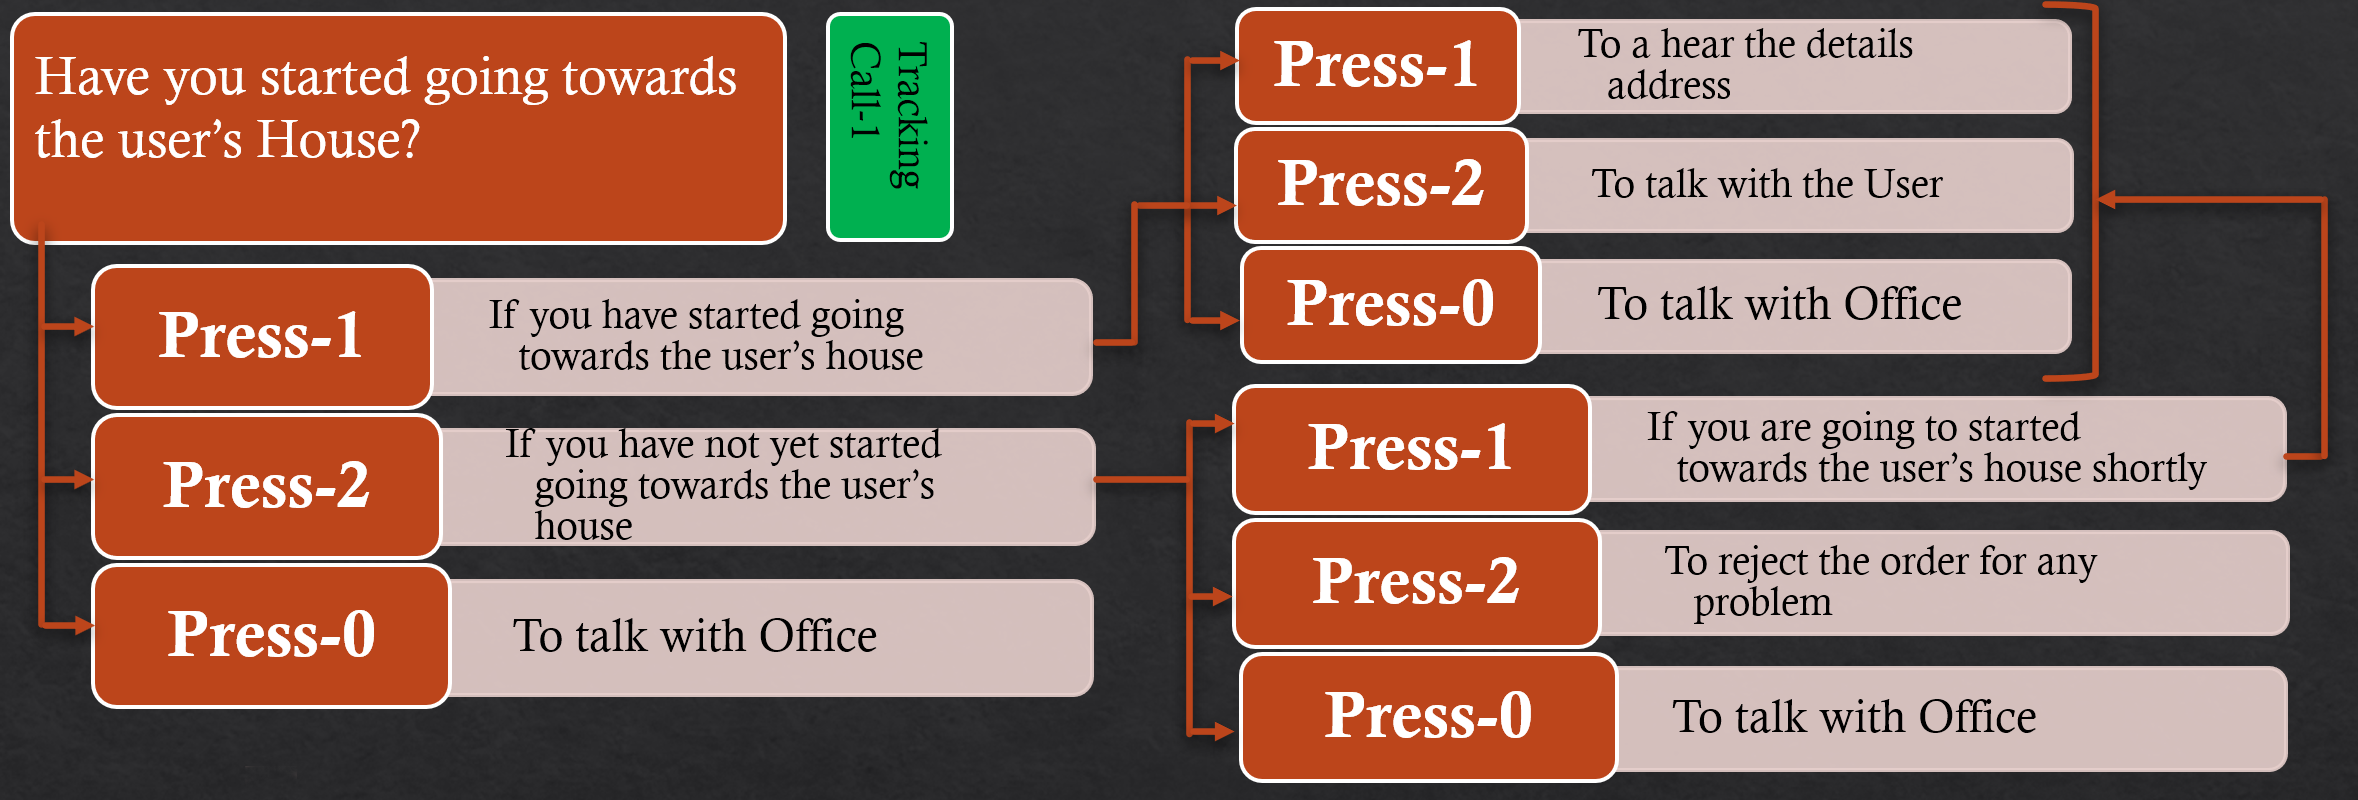
\includegraphics[width=0.9\linewidth]{images/ivrflow.png}
  \caption{The final design of one of the IVR menus, created by \PC{} in Microsoft Powerpoint.}\label{fig:ivrFlow}
  \Description{A cropped screenshot of a PowerPoint slide, showing a series of text boxes connected by arrows representing an IVR menu system. The first box reads 'Have you started going towards the user's house?', and is connected to three smaller boxes, reading: 'Press 1 if you have started going towards the user's house'; 'Press 2 if you have not yet started going towards the user's house; 'Press 0 to talk to the office'. The first two options are connected to submenus. The options of the first submenu read: 'Press 1 to hear the detailed address'; 'Press 2 to talk with the user'; 'Press 0 to talk with the office'. The second submenu, where they haven't left yet, has the options: 'Press 1 if you are going to start towards the user's house shortly'; 'Press 2 to reject the order for any problem'; 'Press 0 to talk with office.' Pressing the first option in this submenu sends the user to the other submenu.}\label{fig:ivrFlow}
\end{figure*}

\item \textit{An operational prototype}, which aimed to actualise and test the IVR process. In-lieu of a fully automated IVR system, \PC{} used human call operators who followed the algorithmic recommendations and the designed IVR script to contact and interact with the domestic workers. Dubbed the `Human IVR', this stage reproduced a `Wizard of Oz'-style prototype, supplanting all local guides who had previously been employed by the company. Workshop discussions during this stage focused on this prototype's implementation, how it was performing, and what feedback \PC{} had received about it from the domestic workers.

A design ethnographer on the research team introduced an additional reflexive lens to these workshops to explore how the priorities and values of each stakeholder were reflected in discussions, and how priorities were negotiated and reflected in design decisions. This research was carried out through observations of the workshops (or workshop recordings), and semi-structured interview discussions both during or after the workshops. 
\end{enumerate}

\subsection{Data collection and analysis}

In order to portray how the values and motivations of the design partners impacted the IVR's design, this paper uses the produced artefact as a lens through which we go on to discuss how the values and priorities of each design partner were negotiated and represented, and how such findings had practical consequences in the final design. As such, our analysis particularly focused on the decisions and negotiations surrounding the system's key features. Data used in the analysis included: (i) recordings of workshop discussions and interviews that were transcribed; (ii) notes taken by researchers during workshops; and (iii) visual diagrams of the iterations of the IVR flow (e.g. Figure \ref{fig:ivrFlow}). 

Data analysis involved three iterative stages: (i) the final IVR flow design was analysed to identify the specific points in a job cycle that domestic workers interacted directly with the IVR system; (ii) workshop transcriptions and meeting notes were then read multiple times to identify dialogue that directly or indirectly informed how and why workers would interact with the IVR system at each point; and (iii) dialogue between each stakeholder was screened for values and motivators that were surfaced and subsequently negotiated through this iterative process. 

\subsection{Researcher Positionality and Influence}

The study's two lead researchers are not Bangladeshi or women of colour. In an attempt to mitigate the impact of cultural biases and contextual misunderstandings, this paper's three Bangladeshi authors often participated in discussions with the design partners and were frequently consulted by the other members of the research team. To avoid an overbearing influence upon the design and resulting ethnographic data, the researchers' design suggestions were usually presented to the design partners as valid alternatives, rather than being definitively better options. The exceptions to this were when the existing design had the potential to cause harm or endanger the domestic workers (such as the system giving the workers' phone numbers to clients, see Section \ref{sec:JobOffer}). All changes to the design in each iteration were made by \PC{} after having received feedback from \NGO{} and the research team.